\section{Мета і програмні засоби}
\label{sec:objective}

\subsection{Мета}

Метою цієї лабораторної роботи є дослідження практичної реалізації криптографічних механізмів у протоколі 
Transport Layer Security (TLS), вивчення принципів встановлення безпечного з'єднання, розгляд використання 
цифрових сертифікатів та аналіз заходів захисту від атак на безпечний канал зв'язку.

Зокрема, я для себе викоремив наступні завдання:
\begin{enumerate}[label=\arabic*.]
    \item Практичне дослідження з'єднань TLS із мінімум двома (я обрав 3) загальнодоступними веб-сайтами
    \item Аналіз сучасних механізмів безпеки TLS за допомогою аналізу низки технічних характеристик.
    \item Поглиблене дослідження уразливості TLS через атаку POODLE (CVE-2014-3566).
    \item Аналіз сценарію порушення безпеки, пов'язаного з вимкненою перевіркою сертифікатів.
\end{enumerate}

\subsection{Програмні засоби}

Для дослідження з'єднань TLS, я на свому комп'ютері з ОС Windows 10 використовував наступні інструменти:
\begin{itemize}
    \item \textbf{Web Browser (Google Chrome)} -- вбудований переглядач сертифікатів (F12 $\rightarrow$ вкладка 
        «Безпека») дозволяє перевірити сертифікат сервера, його ланцюжок, набір шифрів та версію TLS, узгоджену для 
        поточного HTTPS-з'єднання.
    \item \textbf{OpenSSL} (через Powershell (можна і в Bash)) -- утиліта командного рядка openssl 
        \texttt{openssl s\_client} підключається до віддаленого сервера та відображає повний стенограму \\ 
        TLS-рукостискання, узгоджений набір шифрів, ланцюжок сертифікатів та деталі сертифіката~\cite{openssl_docs}. Приклад використання:
\end{itemize}

\begin{minted}[fontsize=\small, breaklines]{bash}
    openssl s_client -connect google.com:443 -servername google.com
    openssl s_client -connect google.com:443 -servername google.com | openssl x509 -noout -text
\end{minted}

Додатково, ще знайшов онлайн-ресурс для перевірки TLS конфігурації:
\begin{itemize}
    \item \textbf{SSL Labs Server Test} (\url{https://www.ssllabs.com/ssltest/}) -- онлайн-інструмент, що виконує 
    комплексний аналіз конфігурації TLS сервера, підтримуваних протоколів, наборів шифрування та відомих вразливостей.
\end{itemize}

\section{TLS Connection Research}
\label{sec:task1}

Для свого дослідження я обрав три загальнодоступні веб-сайти, розташовані в США:
\begin{enumerate}
    \item \textbf{google.com} --- глобальний постачальник технологій та найбільша пошукова система;
    \item \textbf{amazon.com} --- чи ненайбільша комерційна платформа;
    \item \textbf{nist.gov} --- Національний інститут стандартів і технологій США, урядовий ресурс.
\end{enumerate}

Цим вибором я хотів забезпечити різноманітність у різних секторах (технології, електронна комерція, уряд) та
різних центрах сертифікації.

\subsection{Параметри сертифікатів та самого з'єднання}

У таблицях~\ref{tab:tls_params} і~\ref{tab:cert_params} я зібрав підсумкові дані щодо параметрів з'єднання TLS
та сертифікатів, отриманих для кожного веб-ресурсу.

\begin{figure}[ht]
    \centering
    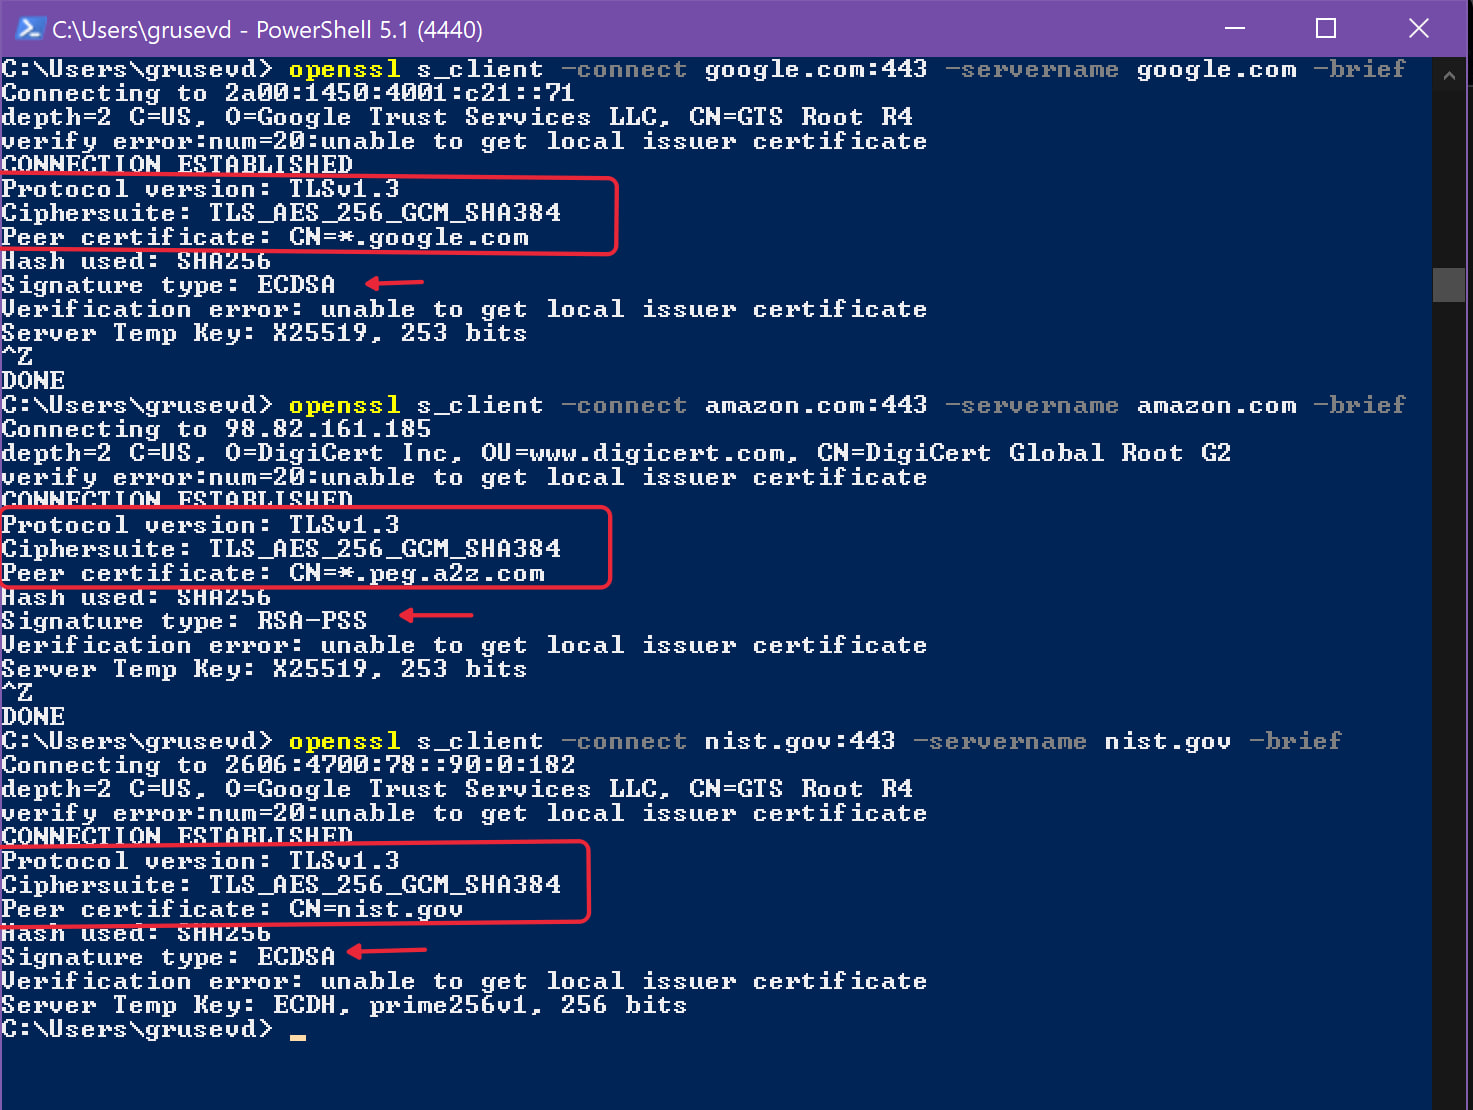
\includegraphics[width=0.85\linewidth]{pic/chains_and_ciphers.jpg}
    \caption{Вивід команди OpenSSL \texttt{s\_client} для google.com, amazon.com та nist.gov}
\end{figure}

\begin{table}[!htbp]
    \centering
    \begin{tblr}{
        colspec = {X[1.2,l] X[1,l] X[1,l] X[1,l]},
        row{1} = {font=\bfseries\small, bg=gray!15},
            hlines, vlines,
            rowsep = 3pt,
            }
            Параметр      & google.com            & amazon.com     & nist.gov      \\
            Версія TLS    & TLS 1.3               & TLS 1.3        & TLS 1.2 / 1.3 \\
            Набір шифрів  & {TLS\_AES\_256\_GCM\_                                  \\SHA384} & {TLS\_AES\_128\_GCM\_\\SHA256} & {TLS\_AES\_256\_GCM\_\\SHA384} \\
            Обмін ключами & X25519 (ECDHE)        & X25519 (ECDHE) & ECDHE         \\
            {Forward                                                               \\Secrecy} & Так & Так & Так \\
            HSTS          & Так                   & Так            & Так           \\
            {Прозорість                                                            \\Сертифікатів} & Так (SCTs) & Так (SCTs) & Так (SCTs) \\
    \end{tblr}
    \caption{Параметри TLS-з'єднання для досліджуваних веб-сайтів}
    \label{tab:tls_params}
\end{table}

\begin{table}[!htbp]
    \centering
    \caption{Параметри цифрових сертифікатів для досліджуваних веб-сайтів}
    \label{tab:cert_params}
    \begin{tblr}{
            colspec = {X[1.2,l] X[1,l] X[1,l] X[1,l]},
            row{1} = {font=\bfseries\small, bg=gray!15},
            hlines, vlines,
            rowsep = 3pt,
        }
        Параметр             & google.com                                    & amazon.com                                     & nist.gov                                      \\
        Ім'я суб'єкта (CN)   & *.google.com                                  & www.amazon.com                                 & *.nist.gov                                    \\
        Емітент (Issuer)     & {Google Trust                                                                                                                                  \\Services (WR2)} & {Amazon RSA\\2048 M04} & {DigiCert TLS RSA\\SHA256 2020 CA1} \\
        {Public Key                                                                                                                                                           \\Algorithm} & ECDSA P-256 & RSA 2048-bit & RSA 2048-bit \\
        {Алгоритм підпису}   & {ECDSA with                                                                                                                                    \\SHA-256} & {SHA-256 with\\RSA} & {SHA-256 with\\RSA} \\
        Термін дії           & {Sep 28, 2026 -- Dec 21, 2026} $\sim$3 months & {Jan 19, 2026 -- Jan 12, 2027} $\sim$12 months & {Oct 22, 2026 -- Jan 20, 2027} $\sim$3 months \\
        {Використання ключа} & {Digital Signature}                           & {Digital Signature,                                                                            \\Key Encipherment} & {Digital Signature,\\Key Encipherment} \\
        {SAN (selected)}     & {*.google.com,                                                                                                                                 \\*.youtube.com,\\google.com, ...} & {www.amazon.com,\\amazon.com,\\*.pci.amazon.com} & {*.nist.gov,\\nist.gov} \\
    \end{tblr}
\end{table}

\begin{figure}[!ht]
    \centering
    \begin{minipage}{0.47\linewidth}
        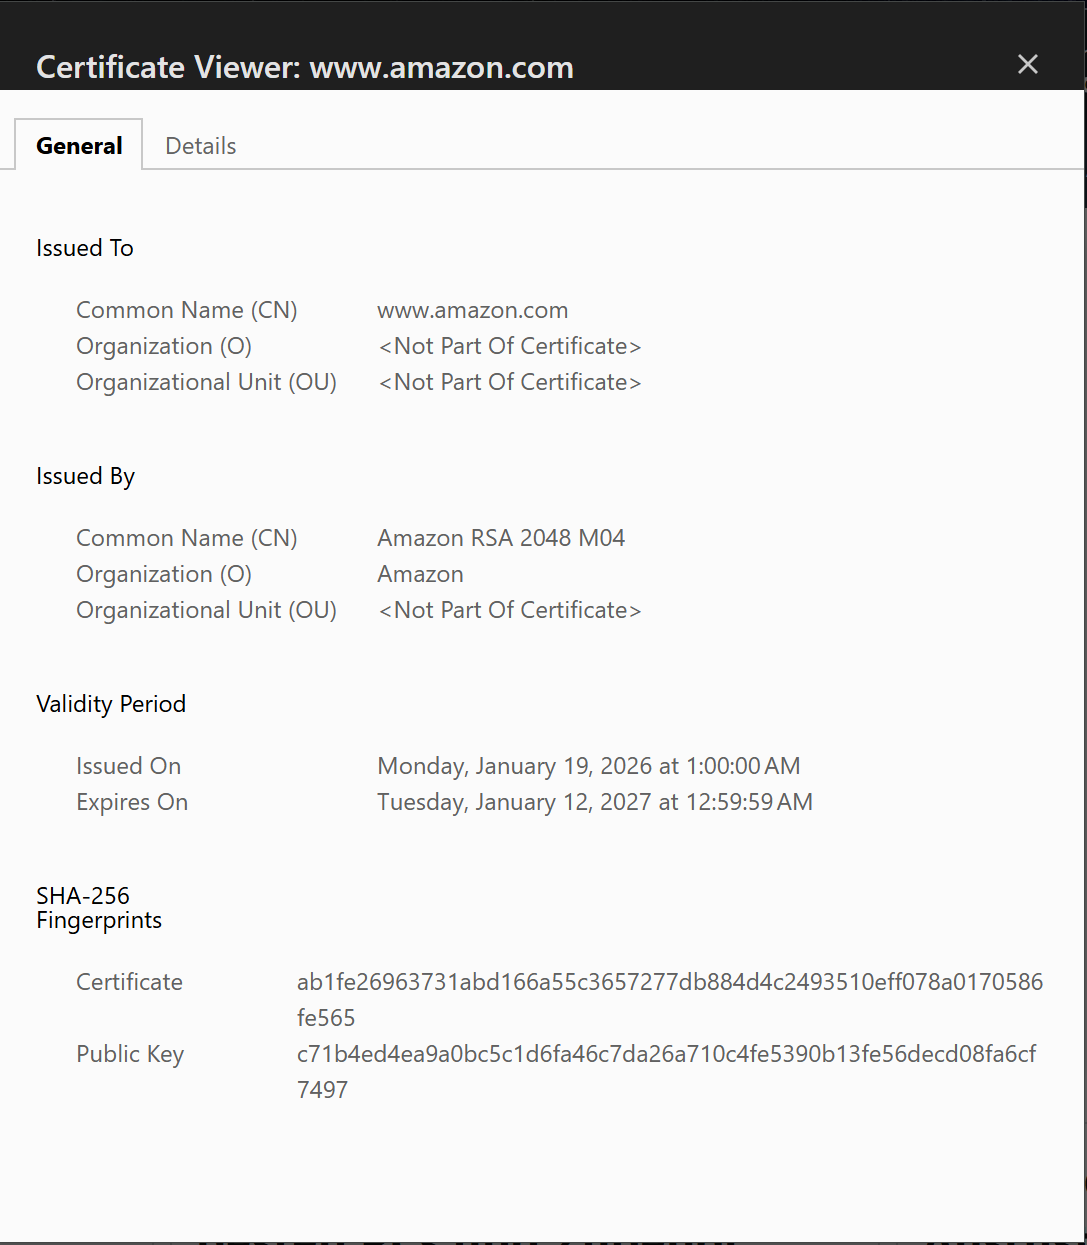
\includegraphics[width=0.75\linewidth, scale = 0.5]{pic/amazon.jpg}
    \end{minipage}
    \begin{minipage}{0.47\linewidth}
        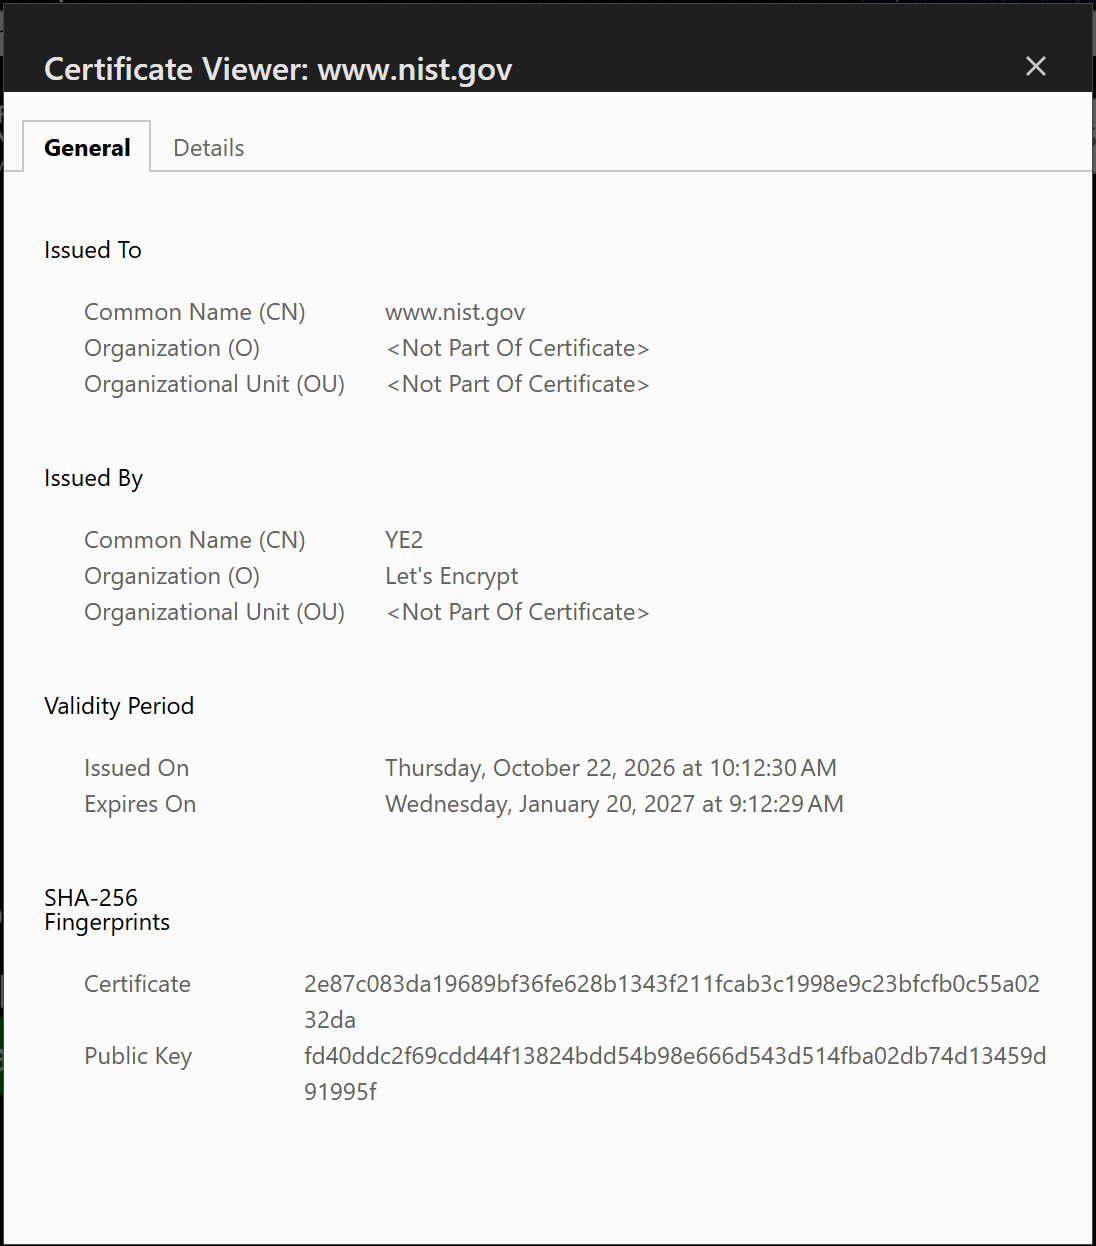
\includegraphics[width=0.75\linewidth]{pic/nist.jpg}
    \end{minipage}
    \caption{Chrome certificate viewer for amazon.com. \& nist.gov}
\end{figure}

\subsection{Subject Alternative Name (SAN)}

Розширення Subject Alternative Name «Альтернативна назва суб'єкта» (скорочено SAN), визначене в RFC~5280~\cite{rfc5280}, 
дозволяє одному сертифікату захищати кілька доменних імен. Наприклад, той же сертифікат Google охоплює понад 100 SAN, 
включаючи \texttt{*.google.com}, \texttt{*.youtube.com}, \texttt{*.googleapis.com}, та власне \texttt{google.com}. 
Це замінює старий підхід Common Name (CN). SAN є основним механізмом перевірки імені хоста, який використовують 
сучасні браузери. Якщо у полі "Додаткові імена підписувача"{} (SAN entry) відсутній відповідний запис, браузер 
відхилить сертифікат, незважаючи на те, що CN збігається із запитуваним ім'ям хоста.

\subsection{Сертифікатний ланцюг (Certificate Chain)}

Кожен досліджуваний веб-сайт має власний ланцюжок з сертифікатів, який встановлює довіру від сертифіката сервера 
до кореневого центру сертифікації (root CA), якому довіряє операційна система або браузер:

\begin{itemize}
    \item \textbf{google.com}: Сертифікат сервера (*.google.com) $\to$ GTS CA 2A3 (проміжний, Google Trust Services) 
        $\to$ GTS Root R1 (root CA)~\cite{google_trust_services}.
    \item \textbf{amazon.com}: Сертифікат сервера (www.amazon.com) $\to$ Amazon RSA 2048 M04 (проміжний) $\to$ 
        Amazon Root CA~1 (root CA)~\cite{amazon_trust_services}.
    \item \textbf{nist.gov}: Сертифікат сервера (*.nist.gov) $\to$ DigiCert TLS RSA SHA256 2020 CA1 (проміжний) 
        $\to$ DigiCert Global Root CA (root CA).
\end{itemize}

Проміжні центри сертифікації мають взаємне підписання або попередньо встановлені зв'язки в сховищах довіри, що 
дозволяє клієнтам формувати ланцюг довіри без необхідності безпосереднього знання кожного CA-емітента. Ця 
ієрархічна модель, визначена в RFC~5280~\cite{rfc5280}, є основою web-PKI (Web Public Key Infrastructure).

\subsection{TLS "рукостискання" (Handshake Process)}

\begin{figure}[!htbp]
    \centering
    \begin{tikzpicture}[
        box/.style = {draw, rounded corners, minimum width=2.6cm, minimum height=0.7cm, font=\small\sffamily},
        arrow/.style = {-{Stealth[length=5pt]}, thick},
        >=Stealth
        ]
        % Actors
        \node[box, fill=blue!10] (client) at (1, 0) {Client};
        \node[box, fill=green!10] (server) at (9, 0) {Server};

        % Draw vertical lifelines
        \draw[thick, gray!40] (1, -0.4) -- (1, -10.2);
        \draw[thick, gray!40] (9, -0.4) -- (9, -10.2);

        % ClientHello
        \draw[arrow, blue!70] (1, -1.2) -- node[above, font=\scriptsize] {ClientHello} (9, -1.2);
        \node[font=\scriptsize, text width=6.5cm, align=center] at (5, -1.7) {supported versions, cipher suites, key\_share (ECDHE)};

        % ServerHello + Finished
        \draw[arrow, green!60!black] (9, -2.4) -- node[above, font=\scriptsize] {ServerHello} (1, -2.4);
        \draw[arrow, green!60!black] (9, -3.1) -- node[above, font=\scriptsize] {Encrypted Extensions} (1, -3.1);
        \draw[arrow, green!60!black] (9, -3.8) -- node[above, font=\scriptsize] {Certificate + CertificateVerify} (1, -3.8);
        \draw[arrow, green!60!black] (9, -4.5) -- node[above, font=\scriptsize] {Finished} (1, -4.5);

        % Note about encryption
        \draw[decorate, decoration={brace, amplitude=5pt}] (9.3, -2.3) -- (9.3, -4.5) node[midway, right=6pt, font=\scriptsize, text width=2.2cm] {All encrypted with handshake keys};

        % Key derivation note
        \draw[thick, orange!70, densely dotted] (0.5, -5.0) -- (9.5, -5.0);
        \node[font=\scriptsize\itshape, text=orange!70!black, anchor=east] at (0.4, -5.0) {Keys derived};

        % Client Finished
        \draw[arrow, blue!70] (1, -5.6) -- node[above, font=\scriptsize] {Finished} (9, -5.6);

        % Application data
        \draw[arrow, blue!70, dashed] (1, -6.4) -- node[above, font=\scriptsize] {Application Data (encrypted)} (9, -6.4);
        \draw[arrow, green!60!black, dashed] (9, -7.0) -- node[above, font=\scriptsize] {Application Data (encrypted)} (1, -7.0);

        % Labels
        \node[font=\scriptsize\itshape, text=red!70!black] at (5, -7.7) {Handshake complete in 1 round trip};

    \end{tikzpicture}
    \caption{Simplified TLS 1.3 handshake (1-RTT)}
    \label{fig:tls13_handshake}
\end{figure}

Взаємодія рукостискань TLS~1.3~\cite{rfc8446}, зображена на рисунку~\ref{fig:tls13_handshake}, забезпечує встановлення 
безпечного з'єднання за один цикл обміну даними (1-RTT), що є значним покращенням порівняно з двома циклами обміну даних, 
як це було в TLS 1.2. Цей процес забезпечує три ключові властивості безпеки:

\begin{enumerate}
    \item \textbf{Server authentication}: Сервер підтверджує свою ідентичність, надаючи сертифікат, підписаний 
        довіреним центром сертифікації (CA) генеруючи повідомлення \texttt{CertificateVerify}, яке підтверджує 
        наявність відповідного приватного ключа.
    \item \textbf{Cryptographic parameter negotiation}: Повідомлення \texttt{ClientHello} включає в себе набори 
        шифрів та підтримувані способи обміну ключами. Сервер обирає найнадійніші з параметрів, що підтримуються 
        обома сторонами, і відповідає, надіславши свою частку ключа.
    \item \textbf{Key material derivation}: Обидві сторони здійснюють обмін ключами використовуючи алгоритм 
        Elliptic Curve Diffie-Hellman Ephemeral (ECDHE). Зі спільного секрету за допомогою схеми виведення ключів 
        на основі функції виведення ключів на основі HMAC (HMAC-based Key Derivation Function), виводяться окремі 
        ключі для встановлення з'єднання та трафіку додатків. Також є важливим те, що використовуються тимчасові 
        ключі, що забезпечує пряму секретність~\cite{cloudflare_forward_secrecy}.
\end{enumerate}

\section{Аналіз сучасних механізмів протоколу TLS}
\label{sec:task2}

\subsection{Ключові відмінності між TLS 1.3 та TLS 1.2}

TLS~1.3, станадартизований у RFC~8446~\cite{rfc8446}, вносить фундаментальні зміни порівняно з TLS~1.2~\cite{rfc5246}.
Тож, закинувши ці два документи в ШІ, я отримав наступне порівняння:

\begin{table}[!htbp]
    \centering
    \begin{tblr}{
            colspec = {X[1.2,l] X[1,l] X[1,l]},
            row{1} = {font=\bfseries\small, bg=gray!15},
            hlines, vlines,
            rowsep = 3pt,
        }
        Змінена складова             & TLS 1.2                  & TLS 1.3                     \\
        Затримка з'єднання (latency) & 2-RTT                    & 1-RTT (+ 0-RTT resumption)  \\
        Набори шифрів                & 37+ (including insecure) & 5 AEAD-only suites          \\
        Обмін ключами                & RSA, DHE, ECDHE          & ECDHE only (X25519, P-256)  \\
        Режими шифрування            & CBC, stream, AEAD        & AEAD only (GCM, ChaCha20)   \\
        Пряма секретність            & Optional                 & Mandatory                   \\
        Шифрування рукостискань      & Plaintext                & Encrypted after ServerHello \\
        Відновлення                  & Session ID / ticket      & PSK-based                   \\
    \end{tblr}
    \caption{Порівняння TLS 1.2 і TLS 1.3}
    \label{tab:tls_comparison}
\end{table}

Найбільш значущими змінами є примус до обов'язкового використання прямої секретності (forward secrecy), шляхом 
усунення статичного обміну ключами RSA (RSA key exchange), скорочення наборів шифрів до п'яти варіантів на основі 
AEAD та зашифрований обмін даними (handshakes), що приховують сертифікат сервера від пасивних зловмисників, які 
намагаються перехопити дані~\cite{rfc8446}.

\subsection{Чому зараз вже не можна використовувати SSL та ранні версії TLS?}

SSL~2.0, SSL~3.0~\cite{rfc6101}, TLS~1.0, і TLS~1.1 містять фундаментальні криптографічні слабкості, які неможливо 
усунути за допомогою налаштувань:

\begin{itemize}
    \item \textbf{SSL 3.0}: вразливий до атак типу POODLE (CVE-2014-3566), які використовують недетерміноване 
        CBC padding~\cite{poodle_paper}. У самому протоколі немає виправлення цього недоліку.
    \item \textbf{TLS 1.0}: вразливий до атаки BEAST (ланцюгове з'єднання векторів ініціалізації CBC) та 
        використовує MD5-SHA-1 у своїй Pseudo-Random Function (PRF).
    \item \textbf{TLS 1.1}: Хоча в ньому виправлено вищезгадану проблему з ланцюгом векторів ініціалізації (IV), 
        він все ще підтримує слабкі набори шифрів такі як RC4, 3DES, не вимагає шифрування AEAD, а його PRF 
        базується на MD5 та SHA-1.
\end{itemize}

Стандарт RFC~8996~\cite{rfc8996} офіційно визнає TLS 1.0 та 1.1 застарілими, а NIST~SP~800-52~Rev.~2~\cite{nist_sp800_52r2} 
у свою чергу встановлює TLS~1.2 як мінімальний стандарт для федеральних систем США, при цьому наполегливо 
рекомендуючи використовувати TLS~1.3. Усі браузери з 2020 року відключили підтримку цих застарілих версій.

\subsection{Forward Secrecy і як вона захищає від компроментації ключа}

«Forward Secrecy» (також відома як «Perfect Forward Secrecy», PFS) -- це властивість протоколів узгодження 
ключів, що гарантує, що сесійні ключі не можуть бути скомпрометовані, навіть якщо довгостроковий приватний 
ключ сервера згодом стане відомим~\cite{cloudflare_forward_secrecy}.

На практиці це досягається за допомогою обміну ефемерними ключами за алгоритмом Діффі–Хеллмана 
(ephemeral Diffie-Hellman key exchange, DHE або ECDHE): кожна сесія TLS генерує нові, короткочасні пари ключів, які 
використовуються для обчислення спільного секрету, а потім одразу видаляються. Навіть якщо зловмисник запише весь 
зашифрований трафік і згодом отримає приватний ключ сервера, він не зможе відтворити ефемерні ключі і, отже, 
не зможе розшифрувати минулі сесії.

Без даної функції, як і у випадку зі статичним обміном ключами RSA у TLS 1.2, приватний ключ RSA сервера використовується 
безпосередньо для розшифрування pre-master secret. Якщо цей ключ буде скомпрометований внаслідок злому сервера 
або майбутніх відкриттів в криптоаналізі, то усі раніше записані сесії можна буде розшифрувати ретроактивно 
(заднім числом). TLS 1.3 повністю усуває цей ризик, обов'язково застосовуючи ECDHE для всіх з'єднань~\cite{rfc8446}.

\subsection{Certificate Transparency (прозорість сертифікатів)}

Прозорість сертифікатів Certificate Transparency (CT), була визначена вперше у RFC~6962~\cite{rfc6962}, 
являє собою систему публічно перевірювальних журналів, до яких можна лише додавати записи, що фіксують кожен 
сертифікат, виданий учасником системи сертифікації. Її мета -- виявляти неправильно або зловмисно видані сертифікатів. 

\noindent Механізм роботи такий~\cite{google_ct_policy}:
\begin{enumerate}
    \item Центр сертифікації видає сертифікат і надсилає його до одного або кількох журналів CT.
    \item Журнал повертає підписаний часовий штамп сертифіката (Signed Certificate Timestamp, SCT) -- криптографічне 
        підтвердження того, що сертифікат буде включено до журналу протягом визначеного часового вікна (Maximum 
        Merge Delay).
    \item SCT вбудовується в сертифікат (через розширення X.509), передається через розширення TLS або надається
        за допомогою OCSP-степлінгу.
    \item  Браузери (зокрема Chrome з 2018 року) вимагають наявності дійсних SCT з декількох незалежних журналів,
        перш ніж довіряти цьому сертифікату.
    \item Власники доменів та служби моніторингу постійно сканують журнали CT, щоб виявити несанкціоновані
        сертифікати для своїх доменів.
\end{enumerate}

Certificate Transparency виявився вирішальним у виявленні інцидентів, зокрема несанкціонованих сертифікатів Google, 
що прогримів в 2015 році, виданих CNNIC, та скандалу з помилковою видачею сертифікатів Symantec у 2017 році. Наразі 
основні центри сертифікації за замовчуванням надсилають усі сертифікати до журналів CT~\cite{letsencrypt_ct}.

\subsection{CRL та OCSP для перевірки скасування сертифікатів}

Коли сертифікат необхідно анулювати до закінчення його природного терміну дії (через компрометацію ключа, зміну 
політики ЦС або зміну власника домену), існують два механізми для повідомлення про статус анулювання~\cite{rfc5280, rfc6960}:

\textbf{Certificate Revocation Lists (CRL)}~\cite{rfc5280}:
\begin{itemize}
    \item Центр сертифікації періодично публікує підписаний список серійних номерів усіх анульованих сертифікатів.
    \item Клієнти завантажують собі весь список CRL і перевіряють, чи є в ньому серійний номер їхнього сертифіката.
    \item \textit{Обмеження}: списки CRL досягають іноді значних розмірів, оскільки це мільйони записів для великих ЦС, 
        оновлюються вони нечасто (від кількох годин до кількох днів), а їх завантаження спричиняє затримку. Анонімність 
        клієнта збережена.
\end{itemize}

\textbf{Online Certificate Status Protocol (OCSP)}~\cite{rfc6960}:
\begin{itemize}
    \item Клієнт надсилає запит у режимі реального часу до OCSP-відповідача ЦС із серійним номером сертифіката.
    \item Респондер повертає підписаний статус "good"{}, "revoked"{} or "unknown"{}.
    \item \textit{Обмеження}: OCSP створює проблему конфіденційності, оскільки ЦС дізнається, які сайти відвідує 
        клієнт, збільшує затримку для кожного нового TLS з'єднання та створює єдину точку відмови (single failure point) 
        -- якщо респондер недоступний, клієнт повинен або перейти в режим "fail-open"{} (незахищений), або в режим 
        "fail-closed{} (втрата доступності).
\end{itemize}

Технологія \textbf{OCSP Stapling} дозволяє усунути обидві проблеми: сервер періодично фетчить власну OCSP-відповідь 
і "прикріплює"{} її до процесу встановлення з'єднання TLS, завдяки чому клієнту не потрібно звертатися до центру 
сертифікації~\cite{mozilla_server_side_tls}. Однак впровадження цієї технології залишається неповним, і ще 
не всі сервери її реалізують.

\subsection{HTTP Strict Transport Security (HSTS)}

HTTP Strict Transport Security (скорочено HSTS), визначений у стандарті RFC~6797~\cite{rfc6797}, є механізмом політики, за 
допомогою якого веб-сайт вказує браузерам, що взаємодіяти з ним необхідно виключно через HTTPS-з'єднання. Сервер 
повідомляє про цю політику через заголовок HTTP-відповіді \texttt{Strict-Transport-Security}:
\begin{minted}[fontsize=\small]{text}
    Strict-Transport-Security: max-age=31536000; includeSubDomains; preload
\end{minted}

HSTS захищає від таких атак як:
\begin{itemize}
    \item \textbf{SSL stripping}: Зловмисник у мережі перехоплює початковий HTTP-запит і переписує всі HTTPS-посилання 
        на HTTP, змушуючи жертву вважати, що сайт не підтримує шифрування. Якщо HSTS увімкнено, браузер відмовляється 
        надсилати будь-які HTTP-запити на цей домен.
    \item \textbf{Protocol downgrade attacks}: Зловмисник намагається примусово змусити з'єднання використовувати HTTP 
        замість HTTPS. HSTS запобігає цьому, обробляючи всі запити до домену виключно як HTTPS.
    \item \textbf{Cookie hijacking}: Без HSTS файли cookie, встановлені через HTTPS, можуть надсилатися через 
        HTTP, якщо не встановлено прапорець \texttt{Secure}. HSTS примусово використовує HTTPS для всіх запитів, 
        що зменшує цей вектор атаки.
\end{itemize}

Список попереднього завантаження HSTS (який підтримується у Chromium і використовується іншими браузерами) йде ще 
далі -- домени зі списку жорстко задані як такі, що підтримують лише HTTPS, що усуває навіть вікно вразливості під 
час першого відвідування до отримання заголовка HSTS~\cite{rfc6797}. Усі три обрані мною веб-сайти (\texttt{google.com}, 
\texttt{amazon.com}, \texttt{nist.gov}) реалізують HSTS.

\subsection{Необхідність перевірки попри шифрування}

Шифрування саме по собі хоч і забезпечує конфіденційність даних під час передачі, але без перевірки сертифіката
клієнт не має гарантії того, хто саме знаходиться на іншому кінці зашифрованого каналу. Це створює критичну
вразливість! Це відбувається в такі етапи:

\begin{enumerate}
    \item Зловмисник, який здійснюватиме атаку "людина посередині"{} (Man-in-the-Middle, MITM), може пред'явити
        \textit{власний} сертифікат і встановити з клієнтом цілком дійсний зашифрований сеанс TLS.
    \item Одночасно з цим зловмисник встановлює окремий зашифрований сеанс із легітимним сервером.
    \item Дані проходять через зловмисника у вигляді відкритого тексту між двома зашифрованими тунелями, надаючи 
        йому повний доступ для читання та запису до всіх переданих даних
\end{enumerate}

А перевірка сертифіката гарантує, що суб'єкт, який надає сертифікат, є законним "працівником"{} (оператором) даного 
домену. Процес перевірки контролює: 
\begin{enumerate}[label = \arabic*)]
    \item чи підписаний сертифікат довіреним центром сертифікації;
    \item чи збігається SAN сертифіката із запитуваним іменем хоста;
    \item чи не закінчився термін дії сертифіката; 
    \item чи не було сертифікат відкликано. 
\end{enumerate}
Без цих перевірок в реальності шифрування створює хибне відчуття безпеки -- канал шифрується, але сторона на 
іншому кінці може виявитися зловмисником. Цей варіант я детальніше розглянув разом з прикладом у розділі~\ref{sec:task4}.

\section{Вразливості від атаки POODLE}
\label{sec:task3}

\subsection{Заг.огляд}

POODLE (Padding Oracle On Downgraded Legacy Encryption), вразливість у SSL~3.0, шо задокументована як CVE-2014-3566~\cite{poodle_cve}, 
була відкрита співробітниками Google в жовтні~2014~\cite{poodle_paper}. Вона дозволяє активному мережевому зловмиснику 
розшифрувати окремі байти трафіку, зашифрованого за протоколом SSL 3.0 у Cipher Block Chaining (CBC) mode.

\subsection{Технічна складова}

Ця вразливість використовує фундаментальний конструктивний недолік у специфікації CBC padding (заповнення) у 
протоколі SSL~3.0~\cite{rfc6101}:

\begin{itemize}
    \item У протоколі SSL~3.0 режим CBC вимагає заповнення, щоб довести обсяг відкритого тексту до кратного
        розміру блоку (8 байтів для 3DES, 16 байтів для AES).
    \item Саме заповнення може складається з довільних байтів, після яких йде один (значущий для сервера) байт, 
        що вказує на довжину заповнення. І перевіряється саме він. Вразливість протоколу полягає в саме в цьому. 
        Наприклад паддінг довжини 3, останні три байти "AA"{}, "FF"{}, "03"{}, первірятиметься останній.
    \item На противагу цьому, TLS~1.0+ вимагає, щоб усі байти заповнення мали те саме значення, що й байт
    довжини, а одержувач перевіряє кожен байт. Тобто в ідеалі, для уникнення атаки мало би бути "03"{}, "03"{}, "03"{}. 
    Більш детально на прикладі нижче.
\end{itemize}

Ця неповна перевірка створює так званий padding oracle (хз як перекласти), що дозволяє зловмиснику маніпулювати 
блоками шифрованого тексту та спостерігати, чи сервер приймає чи відхиляє змінений запис:

\begin{enumerate}
    \item Зловмисник визначає (підбором) блок шифрованого тексту $C_i$, що містить цільовий байт для розшифрування.
    \item Він замінює останній блок шифрованого тексту (який містить заповнення) на $C_i$.
    \item Оскільки під час розшифрування сервер перевіряє лише останній байт розшифрованого блоку, то з ймовірністю 
        $1/256$, останній байт виявляється дійсною довжиною заповнення (від 0x00 до розміру блоку мінус 1), 
        і запис буде прийнято.
    \item Коли запис приймається, зловмисник може отримати цей байт відкритого тексту за допомогою операції XOR:
    \begin{equation*}
        P_i[\text{last}] = D(C_i)[\text{last}] \oplus C_{i-1}[\text{last}],
    \end{equation*}
    де $D(C_i)[\text{last}]$ відоме значення padding (заповнення). І так далі поки не розшифрує весь текст.
\end{enumerate}

\begin{figure}[!htbp]
    \centering
    \begin{tikzpicture}[
        block/.style = {draw, minimum width=2.2cm, minimum height=0.9cm, font=\small\ttfamily},
        label/.style = {font=\scriptsize\sffamily},
        arrow/.style = {-{Stealth}, thick},
        ]
        % Normal CBC
        \node[font=\small\bfseries\sffamily] at (0, 1) {SSL 3.0 CBC Padding:};

        \node[block, fill=blue!10] (b1) at (0, 0) {Data};
        \node[block, fill=blue!10] (b2) at (2.5, 0) {Data};
        \node[block, fill=orange!20] (b3) at (5, 0) {Data|Pad};
        \node[block, fill=red!15] (b4) at (7.5, 0) {??|len};

        \node[label, below=2pt of b1] {Block 1};
        \node[label, below=2pt of b2] {Block 2};
        \node[label, below=2pt of b3] {Block 3};
        \node[label, below=2pt of b4] {Block 4};

        \draw[decorate, decoration={brace, amplitude=5pt}] (6.3, 0.55) -- (8.7, 0.55) node[midway, above=5pt, font=\scriptsize\sffamily, text=red!60!black] {Only last byte checked!};

        % Attack
        \node[font=\small\bfseries\sffamily] at (0, -2) {POODLE Attack:};

        \node[block, fill=blue!10] (a1) at (0, -3) {Data};
        \node[block, fill=blue!10] (a2) at (2.5, -3) {Target};
        \node[block, fill=blue!10] (a3) at (5, -3) {Data};
        \node[block, fill=yellow!30, draw=red, thick] (a4) at (7.5, -3) {Target};

        \draw[arrow, red, thick] (2.5, -2.3) to[out=-20, in=160] node[midway, above, font=\scriptsize\sffamily, text=red] {copy} (7.5, -2.3);

        \node[font=\small, text=red!60!black, text width=6cm, align=center] at (4, -4.5) {Attacker replaces padding block with the target block. Repeats until server accepts it ($\sim$256 attempts per byte).};

    \end{tikzpicture}
    \caption{POODLE attack: CBC padding oracle in SSL 3.0}
    \label{fig:poodle_attack}
\end{figure}

\subsection{Умови для успішної атаки}

Атака POODLE вимагає виконання наступних умов~\cite{poodle_paper, acunetix_poodle}:

\begin{enumerate}
    \item \textbf{Активність «людини посередині» (Man-in-the-Middle):} зловмисник повинен мати можливість перехоплювати 
        та модифікувати мережевий трафік між клієнтом і сервером (наприклад, у спільній мережі Wi-Fi).
    \item \textbf{Підтримка SSL~3.0. як клієнтом, так і сервером:} навіть якщо обидві сторони підтримують TLS~1.2, 
        зловмисник може змусити здійснити пониження версії протоколу (пункт нижче).
    \item \textbf{Механізм пониження версії протоколу:} зловмисник порушує спроби встановлення з'єднання TLS, змушуючи 
        клієнта перейти SSL~3.0. Цей "фінт вухами"{}, так званий, "downgrade dance"{}, використовує властивість 
        браузерів зворотної сумісності.
    \item \textbf{Можливість ініціювати повторювані запити:} Зловмиснику потрібно, щоб браузер жертви надсилав багато 
        запитів до цільового сервера; зазвичай це досягається шляхом використання JavaScript через HTTP на іншій 
        сторінці (на сусідньому HTTP-сайті або в рекламній мережі).
    \item \textbf{Набір шифрів CBC:} З'єднання має використовувати набір шифрів у режимі CBC (який SSL~3.0 підтримує 
        виключно разом із RC4, що сам по собі є легкокомпроментованим і вразливим)
\end{enumerate}

\subsection{Наслідки атаки}

Успішна атака POODLE дозволяє розшифрувати конфіденційні дані по одному байту зі швидкістю приблизно 256 запитів 
на кожен розшифрований байт. Основними цілями такої атаки виявляються:
\begin{itemize}
    \item Cесійні файли cookie HTTP, що дозволяють перехопити сесію;
    \item Токени автентифікації та токени CSRF;
    \item Частини заголовків або тіл запитів, що містять конфіденційну інформацію.
\end{itemize}

Хоч ця атака і є відносно повільною порівняно з масовим розшифруванням, та для 16-байтового сесійного файлу 
cookie потрібно лише приблизно 4 096 запитів, що є здійсненним за лічені хвилини за сприятливих умов мережі~\cite{poodle_paper}.

\subsection{Заходи щодо зменшення ризику та усунення вразливості}

Вище зазначені вразливості було усунуто за допомогою кількох підходів~\cite{rfc7507, redhat_poodle}:

\begin{enumerate}
    \item \textbf{Вимкнення SSL~3.0}: Усі сучасні браузери та сервери остаточно вимкнули підтримку SSL~3.0.
    \item \textbf{TLS\_FALLBACK\_SCSV} (RFC~7507)~\cite{rfc7507}: Механізм сигналізації, за якого клієнт має право 
        включити спеціальне значення у набір шифрів для пониження версії. Якщо сервер бачить це значення, але підтримує 
        вищу версію протоколу, він відхиляє з'єднання, запобігаючи потенційно можливій атаці.
    \item \textbf{Серверні налаштування}: Всім адміністраторам було рекомендовано негайно вимкнути SSL~3.0 на 
        веб-серверах (Apache: \texttt{SSLProtocol All -SSLv3}; Nginx: \texttt{ssl\_protocols TLSv1.2 TLSv1.3}), але 
        не всі могли дослухатися :)
\end{enumerate}

\subsection{Зв'язок з TLS~1.3}

POODLE \textbf{не є застосовним до TLS~1.3}~\cite{rfc8446}. TLS~1.3 усуває цю вразливість завдяки низці проектних 
рішень:
\begin{itemize}
    \item Набори шифрів CBC повністю видалено; підтримуються лише AEAD (AES-GCM, ChaCha20-Poly1305), що забезпечують автентифікацію 
        всього шифрованого тексту та не мають оракула заповнення (padding oracle).
    \item Механізм захисту від пониження версії вбудовано в протокол: сервер вбудовує контрольне значення у свою відповідь 
        ServerHello, під час узгодження версії, нижчої за  максимальну, що дозволяє клієнту виявляти ненавмисне пониження 
        версії.
    \item SSL~3.0, TLS~1.0, та TLS~1.1 не входять до переліку версій, що узгоджуються в TLS~1.3's (Розширення \texttt{supported\_versions}
        замінює застаріле поле версії).
\end{itemize}

\section{Аналіз сценаріїв порушення безпеки}
\label{sec:task4}

\textit{Ситуація}: Розробник клієнтського застосунку під час встановлення TLS-з'єднання стикається з помилкою 
перевірки цифрового сертифіката сервера. Для усунення помилки він вимикає перевірку сертифіката. Після цього 
TLS-з'єднання успішно встановлюється, і дані між клієнтом і сервером передаються у зашифрованому вигляді.

\subsection*{Чому вимкнення перевірки дозволило встановити з'єднання?}

Помилки перевірки сертифіката виникають, коли бібліотека TLS клієнта не може перевірити сертифікат сервера на 
відповідність власному сховищу довірених сертифікатів. До типових причин належать: сертифікат самопідписаний, 
виданим ненадійним або внутрішнім центром сертифікації, термін дії якого закінчився, або має невідповідність 
імені хосту (запитаний домен не збігається з жодним записом SAN)~\cite{rfc5280}.

Вимкнувши перевірку, розробник дає вказівку бібліотеці TLS пропустити всі перевірки сертифікатів і прийняти 
\textit{будь-який сертифікат}, наданий віддаленою стороною -- незалежно від того, чи є він легітимним, самопідписаним, 
прострочений чи створеним зловмисником. Сам процес встановлення з'єднання TLS (обмін ключами, узгодження шифру, 
налаштування шифрування) відбувається нормально, оскільки ці етапи не залежать від перевірки сертифіката. 
З'єднання функціонує в тому сенсі, що дані передаються у зашифрованому вигляді за протоколом, але фундаментальне 
питання про те, \textit{з ким саме} спілкується клієнт, залишається відкритим.

\subsection*{Які властивості безпеки зберігаються, а які втрачаються?}

\begin{table}[!htbp]
    \centering
    \begin{tblr}{
            colspec = {X[1,l] X[0.8,c] X[0.8,c] X[2,l]},
            row{1} = {font=\bfseries\small, bg=gray!15},
            hlines, vlines,
            rowsep = 3pt,
        }
        Властивість             & Normal TLS & No Verify & Пояснення                                                 \\
        Конфіденційність        & Є          & Часткова  & Зашифровано, але можна буде зламано зловмисником          \\
        Цілісність              & Є          & Часткова  & MAC-protected, але атака MITM може змінювати дані         \\
        Серверна автентифікація & Є          & Відсутня  & Жодного доказу, хто видає себе за сервер                  \\
        Forward Secrecy         & Є          & Є         & ECDHE ключі все ще є тимчасовими                          \\
        Незаперечність          & Часткова   & Відсутня  & Немає прив'язки до фіксованої ідентичності на іншому боці \\
    \end{tblr}
    \caption{Властивості безпеки з перевіркою сертифіката та без неї}
    \label{tab:security_properties}
\end{table}

При вимкненій перевірці сертифікатів \textbf{автентифікація сервера повністю втрачається}. Механізми шифрування та цілісності 
(симетричні шифри, MAC/AEAD-теги) все ще працюють коректно під час передачі даних, але вони захищають канал \textit{лише} 
від пасивних підслуховувачів. У разі активного зловмисника, який здійснює атаку «людина посередині», порушуються 
все -- як конфіденційність, так і цілісність, оскільки зловмисник розриває TLS-з'єднання з обох боків, отримуючи 
доступ до відкритого тексту між двома зашифрованими тунелями.

\subsection*{Чи може зловмисник читати або змінювати дані?}

Є два варіанти зловмисника: перший, це пасивний зловмисник (лише прослуховування) -- він може лише читати, дані 
в мережі все ще зашифровані за допомогою надійних алгоритмів, і без сесійних ключів не може розшифрувати трафік. 
А якщо зловмисник є активним, і здійснює MITM, то так, повністю. Зловмисник надає клієнту власний (підставний) 
сертифікат (який клієнт приймає без перевірки) та окремо підключається до легітимного сервера. Зловмисник розшифровує 
весь трафік від клієнта, читає/змінює його, повторно шифрує та пересилає на сервер. Той самий процес відбувається 
у зворотному напрямку для відповідей сервера. Зловмисник має повний доступ до всіх переданих даних у вигляді відкритого 
тексту.

\begin{figure}[!htbp]
    \centering
    \begin{tikzpicture}[
        box/.style = {draw, rounded corners, minimum width=2.4cm, minimum height=0.8cm, font=\small\sffamily},
        arrow/.style = {-{Stealth}, thick},
        ]
        \node[box, fill=blue!10] (client) at (0, 0) {Client};
        \node[box, fill=red!15, draw=red] (attacker) at (5, 0) {Attacker};
        \node[box, fill=green!10] (server) at (10, 0) {Server};

        \draw[arrow, red!70] (0.8, 0.3) -- node[above, font=\scriptsize] {TLS (attacker's cert)} (4.2, 0.3);
        \draw[arrow, red!70] (4.2, -0.3) -- node[below, font=\scriptsize] {Encrypted to attacker} (0.8, -0.3);

        \draw[arrow, green!60!black] (5.8, 0.3) -- node[above, font=\scriptsize] {TLS (server's cert)} (9.2, 0.3);
        \draw[arrow, green!60!black] (9.2, -0.3) -- node[below, font=\scriptsize] {Encrypted to server} (5.8, -0.3);

        \node[font=\scriptsize\sffamily, text=red!60!black, text width=3cm, align=center] at (5, -1.5) {Plaintext visible here!\\Can read \& modify all data};

        \draw[thick, red, dashed] (5, -0.6) -- (5, -1);
    \end{tikzpicture}
    \caption{MITM attack, коли перевірка сертифікатів вимкнена}
    \label{fig:mitm_attack}
\end{figure}

\subsection*{За яких умов можлива атака MITM?}

Атака MITM стає можливою, коли зловмисник може розміститися на шляху мережі між клієнтом і сервером. За наступних 
умов:
\begin{itemize}
    \item \textbf{Використання публічних мереж Wi-Fi:} Зловмисник, що перебуває в тій самій мережі, може 
        використовувати підробку ARP-пакетів для перенаправлення трафіку через свій пристрій.
    \item \textbf{Зламана мережева інфраструктура:} Зловмисний або зламаний маршрутизатор, комутатор або 
        DNS-сервер може перенаправляти трафік до лап зловмисника.
    \item \textbf{DNS spoofing or hijacking:} Зловмисник перенаправляє доменне ім’я на свою власну IP-адресу.
    \item \textbf{BGP hijacking:} На рівні інтернет-провайдера маніпуляції з маршрутами можуть перенаправити 
        трафік, призначений для діапазону IP-адрес сервера.
    \item \textbf{Зламаний проксі-сервер або використання VPN:} Якщо клієнт маршрутизує трафік через проксі-сервер 
        або VPN, що контролюється зловмисником, весь трафік стає доступним.
\end{itemize}

Якщо перевірка сертифікатів увімкнена, клієнт виявить сертифікат зловмисника і перерве з'єднання. Без неї клієнт 
сліпо довіряє будь-якому сертифікату, який йому надають.

\subsection*{Коректне вирішення проблеми з перевіркою сертифіката}

Замість того, щоб вимкнути перевірку, розробник мав би виявити та усунути першопричину помилки сертифіката:

\begin{enumerate}
    \item \textbf{Expired cертифікат:} Найбанальніше оновити сертифікат сервера у центрі сертифікації (CA).
    \item \textbf{Невідповідність імені хосту (Hostname mismatch):} Переконатися, що SAN сертифіката містить точне 
        ім'я хосту або шаблон із символом підстановки, який клієнт використовує для підключення.
    \item \textbf{Self-signed або internal центр сертифікації:} Встановити кореневий сертифікат центру сертифікації 
        у сховище довіри клієнтського додатка. (під час розробки це було б прийнятним, а у виробничому середовищі --
        ні. Треба було використовувати загальновизнаний центр сертифікації)
    \item \textbf{Incomplete ланцюг сертифікатів:} Налаштувати сервер так, щоб він надсилав повний ланцюг (сертифікат 
        сервера + проміжні CA). Відсутність проміжних сертифікатів вважається поширеною помилкою налаштування.
    \item \textbf{Фіксація сертифіката (Certificate pinning):} Для додатків з високим рівнем безпеки треба було 
        зафіксувати очікуваний сертифікат або відкритий ключ у клієнтському коді, забезпечивши додатковий рівень 
        перевірки, що виходить за межі стандартної моделі довіри до ЦС.
\end{enumerate}

\noindent Ні за яких обставин не слід вимикати перевірку сертифікатів у виробничому коді! Багато мов програмування 
надають зручні, але при цьому небезпечні можливості для цього (наприклад, Python's \texttt{verify=False}, Node.js's 
\texttt{rejectUnauthorized: false}, Java's \texttt{TrustAllCerts}, і т.п.), їх слід позначати під час огляду коду 
як критичні недоліки безпеки, з подальшим виправленням.

\section{Висновки}
\label{sec:conclusions}

Ця лабораторна робота стала для мене практичним дослідженням реалізацій протоколу TLS, поєднавши практичне вивчення 
активних HTTPS-з’єднань з аналізом базових криптографічних механізмів. Дослідження трьох веб-сайтів (google.com, 
amazon.com, nist.gov) продемонструвало, що сучасні сервери переважно використовують TLS~1.3 із наборами шифрів 
AEAD, обов’язковою прямим секретністю через ECDHE та прозорістю сертифікатів. Впровадження компанією Google 
сертифікатів ECDSA та коротких термінів дії (приблизно 90 днів) є підходом, орієнтованим на безпеку, тоді як 
Amazon продовжує використовувати RSA 2048 із довшим терміном дії.

Аналіз механізмів TLS підтвердив, що TLS~1.3 являє собою зміну парадигми в безпеці передачі даних: обов’язкова 
forward secrecy, зменшена latency, зашифровані повідомлення під час встановлення з’єднання та значно спрощений 
набір шифрів усувають цілі класи історичних вразливостей. Уразливість POODLE (CVE-2014-3566) продемонструвала, 
як, здавалося б, незначна помилка в проектуванні протоколу -- недостатня специфікація padding proof CBC у SSL~3.0 
створює реальний вектор атаки. Її дослідження підтверджує принцип, що розробка криптографічних протоколів вимагає 
точної специфікації та рішучої відмови від застарілих версій.

Сценарій перевірки сертифікатів продемонстрував, що шифрування без автентифікації створює лише ілюзію(!) безпеки. 
Безпека TLS вимагає обох елементів: шифрування для захисту даних під час передачі та перевірки сертифікатів, щоб 
гарантувати, що дані дійдуть до призначеного одержувача. Вимкнення перевірки в коді додатка є критичним дефектом 
безпеки, який уможливлює атаки типу "man-in-the-middle"{}(MITM).
